\documentclass[a4paper,12pt]{article}
% ---------------------------------------------------------------------------
% INS3155 Computer Vision - Midterm Project Report (structure of the lecturer's template).
% Compile with XeLaTeX (Overleaf: Menu -> Compiler -> XeLaTeX); the title block contains Vietnamese characters.
% tables/, figures/ and code/ hold the tables, figures and code listings built from the notebook results.
% ---------------------------------------------------------------------------
\usepackage{iftex}
\ifXeTeX
    \usepackage{fontspec}            % Latin Modern (Unicode): also covers Vietnamese characters
\else
    \usepackage[T1]{fontenc}
    \usepackage[utf8]{inputenc}
\fi
\usepackage{geometry}
\usepackage{amsmath,amsfonts,amssymb}
\usepackage{graphicx}
\usepackage{caption}
\usepackage{booktabs}
\usepackage{tabularx}
\usepackage{hyperref}
\usepackage{enumitem}
\usepackage{xcolor}
\usepackage{fancyhdr}
\usepackage{parskip}
\usepackage{fvextra}                 % code appendix: Unicode-safe verbatim with line breaking
\usepackage{float}
\usepackage{tikz}
\usetikzlibrary{arrows.meta,positioning}

% Custom colors
\definecolor{titleblue}{RGB}{0,102,204}
\definecolor{headingblue}{RGB}{0,51,102}
\hypersetup{colorlinks=true, linkcolor=headingblue, citecolor=headingblue, urlcolor=titleblue}

% Page layout
\geometry{top=2.5cm,bottom=2.5cm,left=2.5cm,right=2.5cm}
\setlength{\parindent}{0pt}
\setlength{\parskip}{0.6em}
\setlength{\emergencystretch}{3em}   % let lines with long \texttt{} names stretch instead of overflowing

% Header and footer
\pagestyle{fancy}
\fancyhf{}
\fancyhead[L]{\textbf{INS3155 - Computer Vision Midterm Report}}
\fancyhead[R]{\textcolor{titleblue}{Midterm Project Report}}
\fancyfoot[C]{\thepage}

% Block diagram style
\tikzset{blk/.style={draw, rounded corners, fill=titleblue!8, align=center, minimum height=0.9cm, font=\footnotesize, text width=2.1cm},
         arr/.style={-{Stealth}, thick}}

\begin{document}

% ------------------------------- Title block -------------------------------
\thispagestyle{plain}
\begin{minipage}[c]{0.56\linewidth}
    {\LARGE\bfseries\textcolor{titleblue}{Midterm Project Report}}
\end{minipage}\hfill
\begin{minipage}[c]{0.42\linewidth}
    \centering
    Name: Nguyễn Đình Khải\\
    Student ID: 22070920\\
    Email: \href{mailto:22070920@vnu.edu.vn}{22070920@vnu.edu.vn}
\end{minipage}

\vspace{0.6cm}
\today

\begin{abstract}
This project implements and compares classical, learning-free computer vision techniques for three tasks.
In Part A, Mean, Gaussian and Median filters and Laplacian sharpening are evaluated on two of our own photographs corrupted by Gaussian and salt-and-pepper noise, with $3\times3$, $5\times5$ and $7\times7$ kernels: averaged over both photos, a $3\times3$ median filter is best for salt-and-pepper noise (27.1 dB PSNR), and a $3\times3$ Gaussian filter with $\sigma=1$ for Gaussian noise (26.0 dB), although the best $\sigma$ depends on the image content.
In Part B, the fundamental matrix of the Middlebury \emph{Venus} stereo pair is estimated with RANSAC (0.17 px Sampson error on inliers), and Block Matching (BM) is compared with Semi-Global Block Matching (SGBM) over a grid of parameters: SGBM gives denser and more accurate disparity maps (91.7\% vs.\ 84.6\% valid pixels) at about four times the cost, and its disparity is reprojected into a 3D point cloud.
In Part C, SIFT and ORB are compared on four of our own photographs of a Hanoi street, with RANSAC homographies and feathering: SIFT finds twice as many matches, both reach about 1.5 px inlier RMSE, ORB is nine times faster to detect, and the panorama exposes real ghosting and perspective distortion. As a bonus, Laplacian-pyramid (multi-band) blending with hard-seam masks replaces the semi-transparent ghost of feathering by a single opaque copy on our panorama, and its overlap-sharpness index reaches 99.8\% of the hard seam, against 86.3\% for feathering.
\end{abstract}

% ===========================================================================
\section{Introduction}
Classical computer vision relies on explicit mathematical models: convolution, projective geometry and epipolar geometry. These methods are interpretable, need no training data and run in real time on a CPU, so they remain the backbone of many practical systems, such as denoising and panorama modes in phone cameras, stereo depth sensing for robots and vehicles, and 3D mapping.

The goal of this project is to implement, evaluate and compare classical techniques for three tasks:
\begin{itemize}[nosep]
    \item \textbf{Part A -- Image filtering:} removing noise and sharpening details, the first step of almost every imaging pipeline (camera, medical and surveillance images).
    \item \textbf{Part B -- 3D reconstruction:} recovering the epipolar geometry, a dense disparity map and a 3D point cloud from two views, as used for depth estimation in robotics and autonomous driving.
    \item \textbf{Part C -- Image stitching:} merging four overlapping photos into a panorama, as in phone panoramas and aerial mosaics.
\end{itemize}
Each part compares at least two methods or parameter settings with quantitative metrics (PSNR/SSIM, valid pixels, inlier ratio, RMSE, runtime) and visual inspection. Sections~\ref{sec:A}--\ref{sec:C} present, for each part, the methodology, the implementation and results, and the comparative analysis; Section~\ref{sec:concl} concludes.

\subsection{Experimental Setup}\label{sec:setup}
\textbf{Environment.} Python 3.12 with OpenCV 4.13, NumPy, scikit-image 0.26 (PSNR/SSIM), pandas and Matplotlib, on a Windows 11 laptop CPU. Random steps use a fixed seed (\texttt{seed=42}, \texttt{cv2.setRNGSeed(42)}), so all quality metrics are reproduced exactly. All tables and figures of this report come from one run of the accompanying notebook \texttt{22070920\_NguyenDinhKhai.ipynb}. Runtimes are single measurements after a warm-up call; they vary by roughly $\pm$30\% between runs, so only relative differences should be interpreted.

\textbf{Data.}
\begin{itemize}[nosep]
    \item \textbf{Part A:} two of our own phone photographs. \emph{desk}: a desk (keyboard, notebook, laptop, mouse) in daylight, cropped to remove a laptop screen and rotated to landscape, downscaled to $1024\times635$; it combines high-contrast edges and fine text (white letters on black keys, the notebook cover) with large flat regions (the wooden desk). \emph{setup}: a computer setup (laptop, two monitors, backlit keyboard, mouse, window grille and medals behind), $2568\times1926$ downscaled to $1024\times768$; it has even finer detail (small text on the screens, key legends, thin window bars) next to smooth dark screens and the wooden desk. Each photo is the clean reference; noisy versions are synthesised from it, so PSNR and SSIM are measured against a true clean image. The tables report the mean over the two photos.
    \item \textbf{Part B:} the \emph{Venus} pair of the Middlebury optical-flow benchmark~\cite{baker2011} ($420\times380$) with ground-truth flow. The vertical flow is zero everywhere, so the pair is rectified and the ground-truth disparity of the left image is $d=-u$, within $[-7, 9.4]$ px.
    \item \textbf{Part C:} four of our own photographs of a street in Hanoi (office and apartment buildings, shop fronts, trees, parked and moving vehicles), taken in sequence from left to right from the same spot by rotating a phone (main $1\times$ camera, $2000\times1500$). Each shot is rotated by about 20--25$^\circ$ and the lens covers about 75$^\circ$, so the four photos span roughly 140$^\circ$. Projected onto a single plane, the outer images are then stretched towards infinity: our first attempt on the full photos produced a $12752\times5055$ canvas with SIFT and $22392\times8068$ with ORB, which the program rejects. We therefore keep the central 50\% of the width of each photo ($1000\times1500$), equivalent to a narrower lens; neighbouring crops still overlap by about a third. The original photos are kept in \texttt{data/part\_c/original/}.
\end{itemize}

% ===========================================================================
\section{Part A: Image Filtering}\label{sec:A}
\subsection{Methodology}
\textbf{Noise models.} Additive Gaussian noise: $I_n=\mathrm{clip}(I+\eta)$ with $\eta\sim\mathcal N(0,\sigma_n^2)$ and $\sigma_n=20$ (on the 0--255 scale). Salt-and-pepper noise: each pixel is set to 0 with probability $p/2$ and to 255 with probability $p/2$, with $p=0.05$.

\textbf{Mean (box) filter} replaces each pixel by the average of its $k\times k$ window $W_k$:
\begin{equation}
    \hat I(x,y)=\frac{1}{k^2}\sum_{(i,j)\in W_k} I(x+i,\,y+j).
\end{equation}
\textbf{Gaussian filter} weights the neighbours by their distance to the centre:
\begin{equation}
    G_\sigma(i,j)=\frac{1}{2\pi\sigma^2}\exp\!\left(-\frac{i^2+j^2}{2\sigma^2}\right),\qquad \hat I = G_\sigma * I .
\end{equation}
The kernel is separable into two 1D filters; $\sigma$, not $k$, controls the amount of smoothing as long as $k\gtrsim 6\sigma$.

\textbf{Median filter} is non-linear: $\hat I(x,y)=\operatorname{median}\{I(x+i,y+j) : (i,j)\in W_k\}$. Impulse values (0 or 255) are almost never the median of a window, so they are removed instead of being spread out, and step edges are preserved.

\textbf{Laplacian sharpening} subtracts the second derivative to boost edges:
\begin{equation}
    I_{\text{sharp}} = I - \alpha\,\nabla^2 I,\qquad \nabla^2 I=\frac{\partial^2 I}{\partial x^2}+\frac{\partial^2 I}{\partial y^2}.
\end{equation}
$\nabla^2 I$ is computed with OpenCV's $k\times k$ Laplacian kernels ($k=3,5,7$). Larger kernels have a much larger response (about $4\times$, $64\times$ and $1024\times$ the true second derivative), so each kernel is divided by its response to $f(x,y)=x^2$, whose true Laplacian is 2; the same $\alpha$ then has the same meaning for every $k$. The computation is done in floating point, keeping the sign of the Laplacian, before clipping to $[0,255]$.

\textbf{Metrics.} $\mathrm{MSE}=\frac{1}{N}\sum (I-\hat I)^2$, $\mathrm{PSNR}=10\log_{10}(255^2/\mathrm{MSE})$ and
\begin{equation}
\mathrm{SSIM}(x,y)=\frac{(2\mu_x\mu_y+C_1)(2\sigma_{xy}+C_2)}{(\mu_x^2+\mu_y^2+C_1)(\sigma_x^2+\sigma_y^2+C_2)}~\text{\cite{wang2004}},
\end{equation}
all computed against the clean image, together with the runtime of each filter.

\begin{figure}[H]
\centering
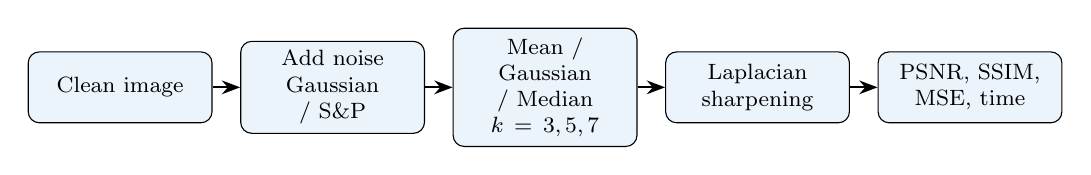
\begin{tikzpicture}[node distance=0.35cm]
\node[blk] (a) {Clean image};
\node[blk, right=of a] (b) {Add noise\\Gaussian / S\&P};
\node[blk, right=of b] (c) {Mean / Gaussian / Median\\$k=3,5,7$};
\node[blk, right=of c] (d) {Laplacian\\sharpening};
\node[blk, right=of d] (e) {PSNR, SSIM,\\MSE, time};
\draw[arr] (a)--(b); \draw[arr] (b)--(c); \draw[arr] (c)--(d); \draw[arr] (d)--(e);
\end{tikzpicture}
\caption{Experimental pipeline of Part A.}
\end{figure}

\subsection{Implementation and Results}
The filters use \texttt{cv2.blur}, \texttt{cv2.GaussianBlur} ($\sigma\in\{0.5,1,2\}$), \texttt{cv2.medianBlur} and \texttt{cv2.Laplacian} ($\alpha\in\{0.5,1\}$), each with $k\in\{3,5,7\}$, i.e.\ 21 settings, all applied to both noise types. Figure~\ref{fig:a_grid} shows, for each noise type, the original, the noisy image, the best setting of each denoising filter, and the best denoised image after Laplacian sharpening ($3\times3$, $\alpha=0.5$).

\begin{figure}[H]
\centering
\includegraphics[width=\linewidth]{figures/part_a/desk_grid.png}
\caption{\emph{desk}: original, noisy, denoised (best setting of each filter) and denoised-then-sharpened images. Top row: Gaussian noise; bottom row: salt-and-pepper noise.}
\label{fig:a_grid}
\end{figure}

\begin{figure}[H]
\centering
\includegraphics[width=\linewidth]{figures/part_a/setup_grid.png}
\caption{\emph{setup}: same layout as Figure~\ref{fig:a_grid}.}
\label{fig:a_grid2}
\end{figure}

\subsection{Comparative Analysis}
\textbf{Quantitative.} Tables~\ref{tab:a_gauss} and~\ref{tab:a_sp} list the metrics of every setting, averaged over the two photos (bold = best), Table~\ref{tab:a_img} gives the best setting of each denoising filter on each photo, and Figure~\ref{fig:a_chart} plots PSNR against the kernel size.

\begin{table}[H]
\centering
\caption{Part A -- Gaussian noise ($\sigma_n=20$), mean over the two photos.}
\label{tab:a_gauss}
\resizebox{0.8\linewidth}{!}{\input{tables/a_metrics_gauss.tex}}
\end{table}

\begin{table}[H]
\centering
\caption{Part A -- salt-and-pepper noise ($p=5\%$), mean over the two photos.}
\label{tab:a_sp}
\resizebox{0.8\linewidth}{!}{\input{tables/a_metrics_sp.tex}}
\end{table}

\begin{table}[H]
\centering
\caption{Part A -- best setting (highest PSNR) of each denoising filter on each photo.}
\label{tab:a_img}
\resizebox{0.7\linewidth}{!}{\input{tables/a_best_per_image.tex}}
\end{table}

\begin{figure}[H]
\centering
\includegraphics[width=0.9\linewidth]{figures/part_a/chart_psnr_vs_kernel.png}
\caption{PSNR versus kernel size for the denoising filters (Gaussian with $\sigma=1$).}
\label{fig:a_chart}
\end{figure}

\textbf{Observations.}
\begin{itemize}
    \item \textbf{Gaussian noise:} on average the Gaussian filter with $\sigma=1$ is best: 26.0 dB with $k=3$, while $k=5,7$ give a slightly lower PSNR (25.6 and 25.5 dB) but the highest SSIM (0.71). It is ahead of the $3\times3$ median (25.2 dB) and mean (25.1 dB) filters. Gaussian noise has small amplitude and affects every pixel, so a weighted average is close to optimal; the median, designed to reject outliers, brings no advantage.
    \item \textbf{The best parameter depends on the image} (Table~\ref{tab:a_img}): on \emph{desk}, $\sigma=1$ wins clearly (27.0 dB against 25.7 dB for $\sigma=0.5$), but on the more detailed \emph{setup} photo the lighter $\sigma=0.5$ gives the highest PSNR (25.5 vs.\ 25.0 dB), because stronger smoothing erases the small screen text and key legends. SSIM still prefers $\sigma=1$ on \emph{setup} (0.69 vs.\ 0.56): PSNR rewards keeping fine detail, SSIM rewards removing the noise in flat regions, so the two metrics can disagree and the filter should be tuned to the content and to the target metric.
    \item \textbf{Salt-and-pepper noise:} the $3\times3$ median filter is far ahead on both photos (27.1 dB and SSIM 0.86 on average, from 17.8 dB for the noisy images; 28.1 dB on \emph{desk}, 26.0 dB on \emph{setup}). Mean and Gaussian filters reach at most 24.0 dB: they \emph{spread} each 0/255 impulse into a grey blob instead of removing it (Figures~\ref{fig:a_grid} and~\ref{fig:a_grid2}, bottom rows).
    \item \textbf{Noise removal vs.\ edge preservation (kernel size):} larger kernels remove more noise but blur edges (over-smoothing). On these sharp photos with many thin edges (key legends, screen text, window bars) the effect is strong: the $7\times7$ median drops to 22.3 dB on salt-and-pepper noise, and on Gaussian noise the $7\times7$ mean falls to 22.0 dB against 25.1 dB for $3\times3$; Gaussian $\sigma=2$ with $k=7$ also loses about 2.4 dB with respect to $\sigma=1$. The Gaussian filter with $\sigma=0.5$ gives \emph{identical} results for every $k$, because the weights outside the central $3\times3$ are almost zero: $\sigma$ sets the smoothing, and $k$ only needs to be about $6\sigma$.
    \item \textbf{Laplacian sharpening and halos:} applied to a noisy image, sharpening lowers PSNR to 13--22 dB, because the second derivative amplifies high-frequency noise; $\alpha=1$ is worse than $\alpha=0.5$, and the larger, smoother $7\times7$ kernel degrades least. After denoising (last columns of Figures~\ref{fig:a_grid} and~\ref{fig:a_grid2}) it makes edges crisper, but it also creates bright/dark \emph{halos} (overshoot) along strong edges and brings back some residual noise, so it should follow denoising and use a small $\alpha$.
    \item \textbf{Runtime} (mean over the two 1024-pixel-wide photos): Gaussian (separable, about 0.6--2 ms) and mean (running sums, about 2--3.7 ms) filters are almost independent of $k$. The median filter goes from about 1 ms ($3\times3$) and 3--4 ms ($5\times5$) to about 70 ms for $7\times7$, because OpenCV switches to a histogram-based algorithm for $k>5$; Laplacian sharpening costs 16--26 ms because of the floating-point arithmetic.
\end{itemize}

\begin{table}[H]
\centering
\caption{Part A -- strengths and weaknesses of each filter.}
\label{tab:a_sw}
\small
\begin{tabularx}{\linewidth}{lXXl}
\toprule
\textbf{Filter} & \textbf{Strengths} & \textbf{Weaknesses} & \textbf{Best for} \\
\midrule
Mean & simple, low computational cost, nearly independent of $k$ & blurs edges, smears impulses & mild Gaussian noise \\
Gaussian & smooth weighting, separable, tunable $\sigma$ & still blurs edges at large $\sigma$ & Gaussian noise \\
Median & removes impulses, keeps step edges & slower for $k>5$, erodes thin lines and corners & salt-and-pepper noise \\
Laplacian & enhances edges and fine detail & amplifies noise, halos for large $\alpha$ & after denoising, small $\alpha$ \\
\bottomrule
\end{tabularx}
\end{table}

% ===========================================================================
\section{Part B: 3D Reconstruction}\label{sec:B}
\subsection{Methodology}
\textbf{Epipolar geometry.} For corresponding points $\mathbf{x}$ (left) and $\mathbf{x}'$ (right) in homogeneous coordinates, the rank-2 fundamental matrix $F$ satisfies
\begin{equation}
    \mathbf{x}'^\top F\,\mathbf{x}=0,\qquad \mathbf{l}'=F\mathbf{x},\quad \mathbf{l}=F^\top\mathbf{x}' ,
\end{equation}
where $\mathbf{l}'$ is the epipolar line of $\mathbf{x}$ in the right image~\cite{hartley2004}. $F$ is estimated using OpenCV RANSAC: repeatedly sample a minimal subset of matches, fit $F$, count the matches closer than a threshold $t$ to their epipolar lines, keep the best model and refit it on all its inliers. Its accuracy is measured by the symmetric point-to-epipolar-line distance and the \textbf{Sampson error}:
\begin{equation}
    d_{\text{epi}}=\tfrac12\!\left(\frac{|\mathbf{x}'^\top F\mathbf{x}|}{\|(F\mathbf{x})_{1:2}\|}+\frac{|\mathbf{x}'^\top F\mathbf{x}|}{\|(F^\top\mathbf{x}')_{1:2}\|}\right),\qquad
    d_{\text{S}}^2=\frac{(\mathbf{x}'^\top F\mathbf{x})^2}{(F\mathbf{x})_1^2+(F\mathbf{x})_2^2+(F^\top\mathbf{x}')_1^2+(F^\top\mathbf{x}')_2^2}.
\end{equation}

\textbf{Disparity.} In a rectified pair, pixel $(x,y)$ of the left image corresponds to $(x-d,y)$ in the right image. \textbf{Block Matching (BM)} picks the $d$ that minimises the sum of absolute differences over a $b\times b$ window (local winner-takes-all). \textbf{SGBM}~\cite{hirschmuller2008} minimises the global energy
\begin{equation}
E(D)=\sum_{\mathbf p} C(\mathbf p,D_{\mathbf p})+\sum_{\mathbf q\in N_{\mathbf p}} P_1\,[|D_{\mathbf p}-D_{\mathbf q}|=1]+\sum_{\mathbf q\in N_{\mathbf p}} P_2\,[|D_{\mathbf p}-D_{\mathbf q}|>1],
\end{equation}
approximately, by aggregating matching costs along several 1D paths:
$L_r(\mathbf p,d)=C(\mathbf p,d)+\min\{L_r(\mathbf p-\mathbf r,d),\,L_r(\mathbf p-\mathbf r,d\pm1)+P_1,\,\min_k L_r(\mathbf p-\mathbf r,k)+P_2\}-\min_k L_r(\mathbf p-\mathbf r,k)$.
We use the usual penalties $P_1=8\cdot3\cdot b^2$ and $P_2=32\cdot3\cdot b^2$: $P_1$ allows slanted surfaces, $P_2$ preserves depth discontinuities.

\textbf{3D reconstruction.} From the disparity, \texttt{cv2.reprojectImageTo3D} computes $[X\,Y\,Z\,W]^\top=Q[x\,y\,d\,1]^\top$:
\begin{equation}
Q=\begin{bmatrix}1&0&0&-c_x\\0&1&0&-c_y\\0&0&0&f\\0&0&1/B&\Delta/B\end{bmatrix}
\ \Rightarrow\ Z=\frac{fB}{d+\Delta},\quad X=\frac{(x-c_x)Z}{f},\quad Y=\frac{(y-c_y)Z}{f}.
\end{equation}
No calibration is supplied with our input files, so $f=420$ px, the left principal point at the image centre and $B=1$ are assumed. We define $\Delta=c_x'-c_x=12$ px as an assumed disparity offset, giving $Z=fB/(d+\Delta)$ for $d=x_L-x_R$. This produces an illustrative point cloud; its shape and metric dimensions are not guaranteed without calibration.

\begin{figure}[H]
\centering
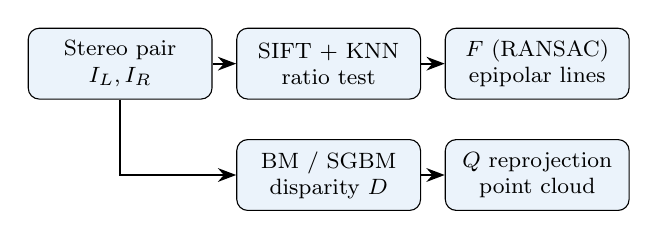
\begin{tikzpicture}[node distance=0.3cm]
\node[blk] (a) {Stereo pair\\$I_L, I_R$};
\node[blk, right=of a] (b) {SIFT + KNN\\ratio test};
\node[blk, right=of b] (c) {$F$ (RANSAC)\\epipolar lines};
\node[blk, below=0.5cm of b] (d) {BM / SGBM\\disparity $D$};
\node[blk, right=of d] (e) {$Q$ reprojection\\point cloud};
\draw[arr] (a)--(b); \draw[arr] (b)--(c); \draw[arr] (a.south) |- (d.west); \draw[arr] (d)--(e);
\end{tikzpicture}
\caption{Pipeline of Part B.}
\end{figure}

\subsection{Implementation and Results}
\textbf{Fundamental matrix.} SIFT keypoints are matched with \texttt{BFMatcher.knnMatch} ($k=2$) and Lowe's ratio test (0.75), and $F$ is estimated with \texttt{cv2.findFundamentalMat(..., cv2.FM\_RANSAC, 1.0, 0.999)}. Figure~\ref{fig:b_epi} draws 15 epipolar lines on \emph{both} images: in each image, the lines of the matching points of the other image pass through the corresponding points.

\begin{figure}[H]
\centering
\includegraphics[width=\linewidth]{figures/part_b/epipolar_lines.png}
\caption{Epipolar lines (SIFT + RANSAC, $t=1$ px). Each colour is one match and its epipolar line.}
\label{fig:b_epi}
\end{figure}

\textbf{Disparity.} \texttt{cv2.StereoBM} (on grey images) and \texttt{cv2.StereoSGBM} (on colour images) are run over \texttt{blockSize} $\in\{5,9,15,21\}$ $\times$ \texttt{numDisparities} $\in\{16,32,48,64\}$, i.e.\ 32 configurations, with \texttt{minDisparity}$=-16$, \texttt{uniquenessRatio}$=10$ and a speckle filter (window 100, range 2). Each map is compared with the ground truth. Figure~\ref{fig:b_disp} shows the best configuration of each method.

\begin{figure}[H]
\centering
\includegraphics[width=\linewidth]{figures/part_b/disparity_comparison.png}
\caption{Colour-coded disparity (same colour scale as the ground truth; white = invalid) and absolute error (0--4 px) of the best BM and SGBM configurations.}
\label{fig:b_disp}
\end{figure}

\textbf{Point cloud.} The best SGBM disparity is reprojected with $Q$; the 1\% nearest and farthest points are discarded as outliers, leaving about 143\,000 coloured points, saved as \texttt{pointcloud\_sgbm.ply} and shown from four viewpoints in Figure~\ref{fig:b_pc}.

\begin{figure}[H]
\centering
\includegraphics[width=0.75\linewidth]{figures/part_b/pointcloud_views.png}
\caption{Point cloud reconstructed from the SGBM disparity, seen from the front, left, right and top.}
\label{fig:b_pc}
\end{figure}

\subsection{Comparative Analysis}
\textbf{Fundamental matrix} (Table~\ref{tab:b_f}). Of 411 ratio-test matches, RANSAC keeps 381 inliers (92.7\%), with a mean epipolar distance of 0.23 px and a Sampson error of 0.17 px on the inliers; over all matches the Sampson error is 1.7 px, which shows how strongly the remaining outliers would bias a non-robust estimate. In Figure~\ref{fig:b_epi} the lines are almost horizontal, as expected for a rectified pair, and pass through the matching points in both images.

\begin{table}[H]
\centering
\caption{Fundamental-matrix estimation with RANSAC (SIFT matches).}
\label{tab:b_f}
\input{tables/b_fundamental.tex}
\end{table}

\begin{table}[H]
\centering
\caption{BM vs.\ SGBM -- best configuration of each method, selected by ``bad$>$2 + inv.'', the percentage of pixels that are invalid or wrong by more than 2 px.}
\label{tab:b_disp}
\setlength{\tabcolsep}{3pt}\resizebox{\linewidth}{!}{\input{tables/b_disparity_best.tex}}
\end{table}

\begin{figure}[H]
\centering
\includegraphics[width=\linewidth]{figures/part_b/chart_stereo_parameters.png}
\caption{Valid ratio, bad-pixel rate and runtime versus \texttt{blockSize} (top, \texttt{numDisparities}=32) and versus \texttt{numDisparities} (bottom, \texttt{blockSize}=9).}
\label{fig:b_sens}
\end{figure}

\textbf{BM vs.\ SGBM} (Tables~\ref{tab:b_disp} and~\ref{tab:b_full}, Figure~\ref{fig:b_sens}).
\begin{itemize}
    \item \textbf{Valid disparity ratio:} the best SGBM map has 91.7\% valid pixels against 84.6\% for the best BM map. BM leaves holes in low-texture areas (the dark poster at the top right) and around depth discontinuities, where the window covers two surfaces. SGBM propagates information through the smoothness terms $P_1, P_2$ and fills these regions.
    \item \textbf{Accuracy:} SGBM is also more accurate (RMSE 0.69 vs.\ 0.85 px, 1.7\% vs.\ 3.0\% of valid pixels wrong by more than 2 px). Counting invalid pixels as errors, 9.9\% of SGBM pixels are bad against 17.9\% for BM.
    \item \textbf{Smoothness and object boundaries:} SGBM surfaces are smooth and its errors concentrate on occlusion boundaries (Figure~\ref{fig:b_disp}, bottom row). BM with a $15\times15$ window shows thicker error bands along depth edges (``foreground fattening'': objects grow by up to half a window).
    \item \textbf{\texttt{blockSize}:} for BM, larger windows increase density (64.7\% at $b=5$ to 84.6\% at $b=15$) but also blur boundaries (bad$>$1 from 1.9\% to 4.4\% at $b=21$). For SGBM, $b\ge15$ \emph{breaks down} (22.6\% bad pixels at $b=15$, and every pixel wrong at $b=21$): the penalties grow with $b^2$ ($P_2=32\cdot3\cdot b^2=21\,600$ at $b=15$ and $42\,336$ at $b=21$, above the 16-bit signed limit of 32\,767). Our hypothesis is that the aggregated path costs then overflow the 16-bit cost type of OpenCV's implementation; we did not verify this inside the library. The OpenCV documentation~\cite{opencv} gives 3--11 as the usual range of \texttt{blockSize}; in our experiments, with penalties proportional to $b^2$, SGBM stays correct up to $b=9$. These configurations are kept as documented failure cases.
    \item \textbf{\texttt{numDisparities}:} with 16 disparities the search range is only $[-16,-1]$ and cannot reach the positive disparities of Venus: BM rejects about half of the pixels (54\% valid) and SGBM assigns wrong values on a large scale (35\% bad pixels). Beyond the needed range ($nd>32$) the invalid band on the left grows (SGBM: 91.6\% $\to$ 84.1\% valid from 32 to 64) and SGBM becomes slower (25 $\to$ 34 ms), because its cost grows linearly with the number of disparities.
    \item \textbf{Runtime:} BM is the fastest (about 5--9 ms) and almost independent of the parameters; SGBM costs about 21--35 ms, roughly four to five times more, which is the price of its global smoothness constraint.
\end{itemize}

\textbf{3D geometry.} The point cloud reproduces the slanted planes of the Venus scene (Figure~\ref{fig:b_pc}): the posters appear as separate tilted planes at different depths. Holes appear where SGBM had no valid disparity, and ``flying pixels'' bridge foreground and background along depth discontinuities, where the disparity is interpolated across the edge. Since $Z\propto 1/(d+\Delta)$, a small disparity error on a distant surface produces a much larger depth error than on a near one. With the assumed camera and offset, this cloud is illustrative; calibration is needed to assess its geometric accuracy.

\begin{table}[H]
\centering
\caption{All BM and SGBM configurations.}
\label{tab:b_full}
\setlength{\tabcolsep}{3pt}\resizebox{\linewidth}{!}{\input{tables/b_disparity_full.tex}}
\end{table}

% ===========================================================================
\section{Part C: Image Stitching}\label{sec:C}
\subsection{Methodology}
\textbf{Features.} \emph{SIFT}~\cite{lowe2004} detects extrema in a Difference-of-Gaussians scale space and describes each keypoint by 128-D histograms of gradient orientations ($4\times4$ cells $\times$ 8 bins), making it invariant to scale and rotation. \emph{ORB}~\cite{rublee2011} combines FAST corners, an orientation from the intensity centroid, and 256-bit rotated BRIEF binary descriptors; it is much faster but less precise.

\textbf{Matching.} Each descriptor of image $i$ is matched to its two nearest neighbours in image $i+1$ ($k=2$; Euclidean L2 distance for SIFT, Hamming distance for the binary ORB descriptors) and kept only if $d_1<0.75\,d_2$ (Lowe's ratio test), which rejects ambiguous matches.

\textbf{Homography.} Two views of a planar scene, or views under pure camera rotation, are related by $\mathbf{x}'\sim H\mathbf{x}$, where $H$ is a $3\times3$ matrix with 8 degrees of freedom (defined up to scale). For pure rotation with the same camera intrinsics, $H=KRK^{-1}$; a planar scene with translation also requires a plane-dependent term. Each correspondence gives two linear equations, so 4 matches determine $H$ by the Direct Linear Transform. RANSAC repeatedly samples 4 matches, fits $H$ and counts the inliers with $\|\mathbf{x}'-\pi(H\mathbf{x})\|<t$, where $\pi$ divides by the third coordinate; it needs
\begin{equation}
N=\frac{\log(1-p)}{\log(1-w^{4})}
\end{equation}
iterations to draw an all-inlier sample with probability $p$ when the inlier fraction is $w$. The best model is refined on all its inliers, and its accuracy is the inlier reprojection RMSE
\begin{equation}
\mathrm{RMSE}=\sqrt{\frac{1}{|\mathcal I|}\sum_{i\in\mathcal I}\|\mathbf{x}'_i-\pi(H\mathbf{x}_i)\|^2}.
\end{equation}

\textbf{Warping and blending.} The middle image is the reference frame, which shortens the homography chains and limits the stretching of the outer images. With $H_{i+1\to i}$ estimated for each adjacent pair, the images are chained to the reference $r$ by $H_{i\to r}=H_{i-1\to r}H_{i\to i-1}$ on the right and $H_{i\to r}=H_{i+1\to r}H_{i+1\to i}^{-1}$ on the left. The canvas is the bounding box of the warped image corners, shifted by a translation $T$ so that all coordinates are positive, and each image is warped with $TH_{i\to r}$. Overlaps are blended by \emph{feathering}:
\begin{equation}
I(\mathbf p)=\frac{\sum_k w_k(\mathbf p)\,I_k(\mathbf p)}{\sum_k w_k(\mathbf p)},
\end{equation}
where $w_k(\mathbf p)$ is the distance from $\mathbf p$ to the border of image $k$ (distance transform), so the weight of each image falls smoothly to zero at its border.

\textbf{Multi-band (Laplacian pyramid) blending (bonus).} Feathering averages the images over the whole overlap, so a moving object or a small misalignment becomes a semi-transparent ghost. Multi-band blending~\cite{burt1983} blends each frequency band over a width proportional to its wavelength. First, a hard seam assigns every pixel to the image with the largest $w_k$, giving binary masks $M_k$. Each warped image is decomposed into a Laplacian pyramid $L_l(I_k)=G_l(I_k)-\mathrm{up}(G_{l+1}(I_k))$, $l=0,\dots,n-1$, with $L_n=G_n$, where $G_l$ is the Gaussian pyramid (blur and subsample by 2). Each band is blended with the mask blurred to the same level, and the panorama is rebuilt from the coarsest level:
\begin{equation}
L_l(I)=\frac{\sum_k G_l(M_k)\,L_l(I_k)}{\sum_k G_l(M_k)},\qquad I=L_0+\mathrm{up}\big(L_1+\mathrm{up}(L_2+\dots)\big).
\end{equation}
Low frequencies (exposure, sky colour) are thus mixed over about $2^n$ pixels and leave no step, while high frequencies (edges, texture) are mixed over only a few pixels around the seam, so details are not averaged across the whole overlap as in feathering. Before building the pyramids, the pixels outside each warped image are filled with the colour of the nearest valid pixel; otherwise the black background would leak into the coarse levels and darken the image borders. With $n=0$ the method reduces to the hard seam without blending.

\begin{figure}[H]
\centering
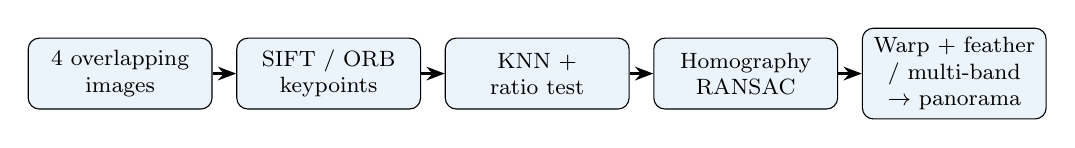
\begin{tikzpicture}[node distance=0.3cm]
\node[blk] (a) {4 overlapping\\images};
\node[blk, right=of a] (b) {SIFT / ORB\\keypoints};
\node[blk, right=of b] (c) {KNN +\\ratio test};
\node[blk, right=of c] (d) {Homography\\RANSAC};
\node[blk, right=of d] (e) {Warp + feather\\/ multi-band\\$\rightarrow$ panorama};
\draw[arr] (a)--(b); \draw[arr] (b)--(c); \draw[arr] (c)--(d); \draw[arr] (d)--(e);
\end{tikzpicture}
\caption{Pipeline of Part C.}
\end{figure}

\subsection{Implementation and Results}
Keypoints come from \texttt{cv2.SIFT\_create} and \texttt{cv2.ORB\_create} (5000 features) and are matched with \texttt{cv2.BFMatcher.knnMatch}. The homography of every adjacent pair is estimated with \texttt{cv2.findHomography(src, dst, cv2.RANSAC, t)} for $t\in\{1,3,5,10\}$ px, and the panorama uses $t=3$ px. Images are warped with \texttt{cv2.warpPerspective}; their footprint masks are eroded by one pixel to drop border pixels interpolated with the black background, and feathering weights come from \texttt{cv2.distanceTransform}. If a pair has fewer than 10 inliers, or the canvas would exceed 30 megapixels (homography chain stretched too far), the program reports it and skips that panorama instead of producing a wrong mosaic. The total stitching time includes detection, matching, RANSAC, warping and blending (feathering). The inputs are the four cropped street photos described in Section~\ref{sec:setup}.

For the blending study (bonus), the SIFT panorama is also blended with a hard seam and with multi-band blending of $n\in\{2,4,6\}$ levels (\texttt{cv2.pyrDown}/\texttt{cv2.pyrUp}; the nearest-pixel filling uses \texttt{cv2.distanceTransformWithLabels}). Without ground truth, two measures are computed on the overlaps (pixels covered by at least two images): the \emph{seam gradient}, the mean Sobel gradient magnitude on the hard-seam line (a visible seam is a step, so a lower value means a less visible seam), and the \emph{overlap sharpness}, the mean $|\nabla^2 I|$ over the overlaps (averaging two misaligned images blurs them and lowers it), also given relative to the hard seam, which copies every pixel from a single image. Figure~\ref{fig:c_blend} enlarges the two $400\times400$ regions where the methods differ most.

\begin{figure}[H]
\centering
\includegraphics[width=\linewidth]{figures/part_c/keypoints_SIFT.png}\\
\includegraphics[width=\linewidth]{figures/part_c/keypoints_ORB.png}
\caption{Keypoints detected by SIFT (top) and ORB (bottom) on the four input images.}
\label{fig:c_kp}
\end{figure}

\begin{figure}[H]
\centering
\includegraphics[width=0.8\linewidth]{figures/part_c/matches_SIFT_pair23.png}\\[2pt]
\includegraphics[width=0.8\linewidth]{figures/part_c/matches_ORB_pair23.png}
\caption{RANSAC inlier matches ($t=3$ px) between images 2 and 3 (top: SIFT, bottom: ORB); at most about 150 lines are drawn.}
\label{fig:c_match}
\end{figure}

\begin{figure}[H]
\centering
\includegraphics[width=\linewidth]{figures/part_c/panorama_SIFT.jpg}
\caption{Final panorama (SIFT + feathering, $5437\times3331$ canvas). Note the stretched left image, the smooth transitions in the sky, and the semi-transparent ``ghost'' motorcyclist in front of the white car on the right.}
\label{fig:c_pano}
\end{figure}

\begin{figure}[H]
\centering
\includegraphics[width=0.8\linewidth]{figures/part_c/panorama_comparison.png}
\caption{Panoramas obtained with SIFT (top) and ORB (bottom).}
\label{fig:c_pano2}
\end{figure}

\begin{figure}[H]
\centering
\includegraphics[width=0.8\linewidth]{figures/part_c/panorama_blending.png}
\caption{Bonus: SIFT panorama blended by feathering (top) and by multi-band blending with 6 pyramid levels (bottom).}
\label{fig:c_pano3}
\end{figure}

\begin{figure}[H]
\centering
\includegraphics[width=0.85\linewidth]{figures/part_c/blending_comparison.png}
\caption{Bonus: enlarged $400\times400$ regions where the methods differ most (canvas coordinates in the first column). Top: a motorcyclist present in only one of the overlapping shots. Bottom: the sky next to the tall building, where the exposure changed between shots.}
\label{fig:c_blend}
\end{figure}

\subsection{Comparative Analysis}
\begin{table}[H]
\centering
\caption{SIFT vs.\ ORB (totals over the three pairs, RANSAC $t=3$ px; total = whole stitching time).}
\label{tab:c_sum}
\setlength{\tabcolsep}{3pt}\resizebox{\linewidth}{!}{\input{tables/c_summary.tex}}
\end{table}

\begin{table}[H]
\centering
\caption{Effect of the RANSAC threshold for each image pair.}
\label{tab:c_thr}
\resizebox{0.75\linewidth}{!}{\input{tables/c_ransac_thresholds.tex}}
\end{table}

\begin{figure}[H]
\centering
\includegraphics[width=0.9\linewidth]{figures/part_c/chart_ransac_threshold.png}
\caption{Inlier ratio (top) and inlier RMSE (bottom) versus the RANSAC threshold, for each image pair.}
\label{fig:c_chart}
\end{figure}

\textbf{Quantitative.}
\begin{itemize}
    \item \textbf{Keypoints and matches:} on these large, textured photos SIFT detects about 8350 keypoints per image, while ORB stops at its 5000 limit; SIFT also yields twice as many ratio-test matches (3213 vs.\ 1622 over the three pairs) and more inliers (1873 vs.\ 1079). Inliers concentrate on the far, static building fa\c{c}ades (Figure~\ref{fig:c_match}); few are found on the road, the moving vehicles and the trees.
    \item \textbf{Inlier ratio and accuracy:} at $t=3$ px only 58\% (SIFT) and 67\% (ORB) of the matches are inliers, far below what an exact homography would give. A homography explains a pure camera rotation; here the phone also moved slightly while turning, so near objects (cars, trees, the pavement) shift differently from the far buildings (parallax), vehicles and people moved between shots, and the facades contain many repeated windows that produce wrong matches. Both detectors reach a similar inlier RMSE (1.48 and 1.49 px): with real photos the error is dominated by these effects rather than by keypoint localisation. ORB's higher ratio comes with half as many matches, clustered on a few high-contrast corners of one facade (air-conditioning units, window frames; Figure~\ref{fig:c_match}), whereas SIFT inliers are spread over the whole building.
    \item \textbf{RANSAC threshold} (Table~\ref{tab:c_thr}, Figure~\ref{fig:c_chart}): the threshold now matters a lot. At $t=1$ px only 18--39\% of the matches are kept, so many correct but slightly imperfect matches are rejected; at $t=10$ px 79--94\% are kept, but RMSE grows from about 0.6 px to 1.8--3.6 px, because points affected by parallax are accepted and the homography becomes a compromise between near and far surfaces. $t=3$ px balances these effects (49--82\% inliers, 1.3--1.8 px RMSE) and is used for the panorama.
    \item \textbf{Runtime:} SIFT detection is about nine times slower than ORB (about 1060 vs.\ 120 ms for four images) and its matching is also slower because it has more descriptors (about 830 vs.\ 340 ms). RANSAC takes less than 10 ms. Most of the time is spent on the large canvas: warping takes about 0.3 s and feathering 2--2.5 s, so the total stitching time is about 4.1 s with SIFT and 3.4 s with ORB.
\end{itemize}

\textbf{Qualitative} (Figures~\ref{fig:c_pano} and~\ref{fig:c_pano2}).
\begin{itemize}
    \item \textbf{Seam visibility and illumination transitions:} feathering leaves no hard seam. The automatic exposure of the phone changed between shots (the sky gets brighter towards the right, where the camera faces the sun); the distance weights turn these differences into smooth gradients across the overlaps instead of visible steps, although no exposure compensation is applied.
    \item \textbf{Geometric alignment:} the static, distant structures are well aligned: the tall building, its windows and bank signs, the shop signs and the trees are continuous across the overlaps, consistent with an RMSE of about 1.5 px.
    \item \textbf{Ghosting:} moving objects produce ghosts. On the right, a motorcyclist who was present in only one of two overlapping shots appears semi-transparent in front of the white car, because feathering averages the two images. With hard-seam masks, multi-band blending replaces this half-transparent copy by an opaque one on our panorama (see below).
    \item \textbf{Perspective distortion:} projecting every image onto the plane of the third image strongly stretches the leftmost image into a large trapezoid (the cars and the tree on the left look much larger), and the canvas ($5437\times3331$ for $1000\times1500$ inputs) has large black wedges. The stretching grows like $\tan\theta$ with the angle from the reference view; with the uncropped photos (about 140$^\circ$ in total) it diverges and no planar panorama can be built. A cylindrical or spherical projection, or photos taken with a narrower field of view, are needed for wide panoramas.
    \item \textbf{SIFT vs.\ ORB:} both give visually equivalent panoramas on this scene. SIFT provides more matches and more inliers, which makes it more robust on difficult image pairs, at a much higher cost; ORB is far faster and, thanks to its many corner features on the facades, accurate enough here.
\end{itemize}

\textbf{Blending: feathering vs.\ multi-band (bonus;} Table~\ref{tab:c_blend}, Figures~\ref{fig:c_pano3} and~\ref{fig:c_blend}\textbf{).}

\begin{table}[H]
\centering
\caption{Bonus: blending methods on the SIFT panorama. Seam gradient: lower = less visible seam; overlap sharpness: mean $|\nabla^2 I|$ on the overlaps (higher = less blur and ghosting).}
\label{tab:c_blend}
\setlength{\tabcolsep}{4pt}\resizebox{0.9\linewidth}{!}{\input{tables/c_blending.tex}}
\end{table}

\begin{itemize}
    \item \textbf{Hard seam:} copying every pixel from a single image keeps the full sharpness but leaves visible steps: the seam gradient is the highest (72.7), the exposure change appears as a sharp line in the sky (Figure~\ref{fig:c_blend}, bottom), and the seam cuts through the motorcyclist and the car (top).
    \item \textbf{Feathering} hides the seams best (seam gradient 44.3), but only because it also blurs everything along them: the overlap sharpness falls to 86.3\% of the hard seam, and the motorcyclist becomes a semi-transparent ghost through which the car is visible.
    \item \textbf{Multi-band blending} combines both advantages: it removes most of the seam step (72.7 $\to$ 50.7 with 4 or 6 levels, a reduction of 30\%) and the sky is smooth, while its overlap-sharpness index reaches 99.8\% of that of the hard seam. On our panorama the motorcyclist is opaque and sharp instead of ghosted; this comes from the hard-seam masks, which take each detail from a single image, combined with the band-limited transition. Two levels already give most of the gain (52.5); beyond four levels the measures no longer change.
    \item \textbf{Limits and cost:} multi-band blending does not choose \emph{where} the seam goes, so it does not remove ghosting in general: a moving object crossed by the seam can still be cut or blurred, as on the cap of the motorcyclist, where a short blurred band remains. These conclusions are limited to this set of photos. A graph-cut seam that avoids moving objects would solve this. It is also about 3.6 times slower than feathering (7.0 vs.\ 2.0 s), because it builds four floating-point pyramids and fills the area outside each image on the 18-megapixel canvas.
\end{itemize}

% ===========================================================================
\section{Conclusion}\label{sec:concl}
\textbf{Key findings.} (1) No filter is best for every noise type: the median filter is clearly superior for impulse noise, while a Gaussian filter with $\sigma\approx0.5$--$1$ is best for Gaussian noise, the exact value depending on how much fine detail the image contains and on the metric (PSNR or SSIM); larger kernels trade edge sharpness for noise removal, and Laplacian sharpening amplifies noise and should only follow denoising with a small $\alpha$. (2) RANSAC estimates the fundamental matrix of the stereo pair with sub-pixel Sampson error. SGBM gives denser, smoother and more accurate disparity than BM at about four times the cost; \texttt{numDisparities} must cover the true disparity range, and with penalties $P_1,P_2$ proportional to $b^2$ the SGBM \texttt{blockSize} must stay small. (3) For stitching real street photos, SIFT finds twice as many matches as ORB, both reach about 1.5 px RMSE, and ORB is about nine times faster to detect. With parallax and moving objects the RANSAC threshold becomes a real trade-off ($t=3$ px is a good compromise), feathering hides seams and exposure changes but leaves ghosts of moving objects, on our panorama, multi-band blending with hard-seam masks replaces these ghosts by opaque copies while still hiding the seams (overlap-sharpness index 99.8\% of the hard seam, 30\% lower seam step), although objects crossed by the seam can still be cut, and a planar projection only works for a limited field of view.

\textbf{Future work.} Edge-preserving filters (bilateral, non-local means) for Part A; calibrating a real camera and capturing our own stereo pair to obtain metric depth, with a left--right consistency check and hole filling, for Part B; a cylindrical projection to keep the full field of view of the photos, exposure compensation, and a graph-cut seam that avoids moving objects, combined with multi-band blending, for Part C.

% ===========================================================================
\section{References}
\begingroup
\renewcommand{\section}[2]{}%      % the numbered heading above replaces the bibliography's own heading
\begin{thebibliography}{9}
\bibitem{opencv} OpenCV Documentation, \url{https://docs.opencv.org/4.x/}.
\bibitem{baker2011} S. Baker, D. Scharstein, J. P. Lewis, S. Roth, M. J. Black, R. Szeliski, ``A Database and Evaluation Methodology for Optical Flow,'' \emph{IJCV}, 92(1):1--31, 2011. Data: \url{https://vision.middlebury.edu/flow/data/}.
\bibitem{hirschmuller2008} H. Hirschmüller, ``Stereo Processing by Semiglobal Matching and Mutual Information,'' \emph{IEEE TPAMI}, 30(2):328--341, 2008.
\bibitem{hartley2004} R. Hartley, A. Zisserman, \emph{Multiple View Geometry in Computer Vision}, 2nd ed., Cambridge University Press, 2004.
\bibitem{lowe2004} D. G. Lowe, ``Distinctive Image Features from Scale-Invariant Keypoints,'' \emph{IJCV}, 60(2):91--110, 2004.
\bibitem{rublee2011} E. Rublee, V. Rabaud, K. Konolige, G. Bradski, ``ORB: An Efficient Alternative to SIFT or SURF,'' \emph{ICCV}, 2011.
\bibitem{burt1983} P. J. Burt, E. H. Adelson, ``A Multiresolution Spline with Application to Image Mosaics,'' \emph{ACM Transactions on Graphics}, 2(4):217--236, 1983.
\bibitem{wang2004} Z. Wang, A. C. Bovik, H. R. Sheikh, E. P. Simoncelli, ``Image Quality Assessment: From Error Visibility to Structural Similarity,'' \emph{IEEE TIP}, 13(4):600--612, 2004.
\end{thebibliography}
\endgroup

% ===========================================================================
\appendix
\section*{Appendix A: Selected Code Listings}
\addcontentsline{toc}{section}{Appendix A: Selected Code Listings}
\setcounter{section}{1}              % subsections are numbered A.1, A.2, A.3
This appendix presents selected functions from the accompanying Jupyter notebook, \texttt{22070920\_NguyenDinhKhai.ipynb}. The complete implementation, input data, experimental results, dependency list, and execution instructions are included in the submission package. To reproduce the experiments, open the notebook from the directory containing \texttt{data/}, select the appropriate Python environment, and run all cells in order. Execution times may vary with the hardware and system load.
\fvset{fontsize=\scriptsize, numbers=left, numbersep=5pt, frame=single, breaklines=true, breakanywhere=true, tabsize=4}
\subsection{Part A: Image Filtering}
\VerbatimInput{code/excerpt_part_a.py}
\subsection{Part B: 3D Reconstruction}
\VerbatimInput{code/excerpt_part_b.py}
\subsection{Part C: Image Stitching}
\VerbatimInput{code/excerpt_part_c.py}

\end{document}
